\documentclass{standalone}
\usepackage{tikz}
\usetikzlibrary{patterns, positioning}


\begin{document}
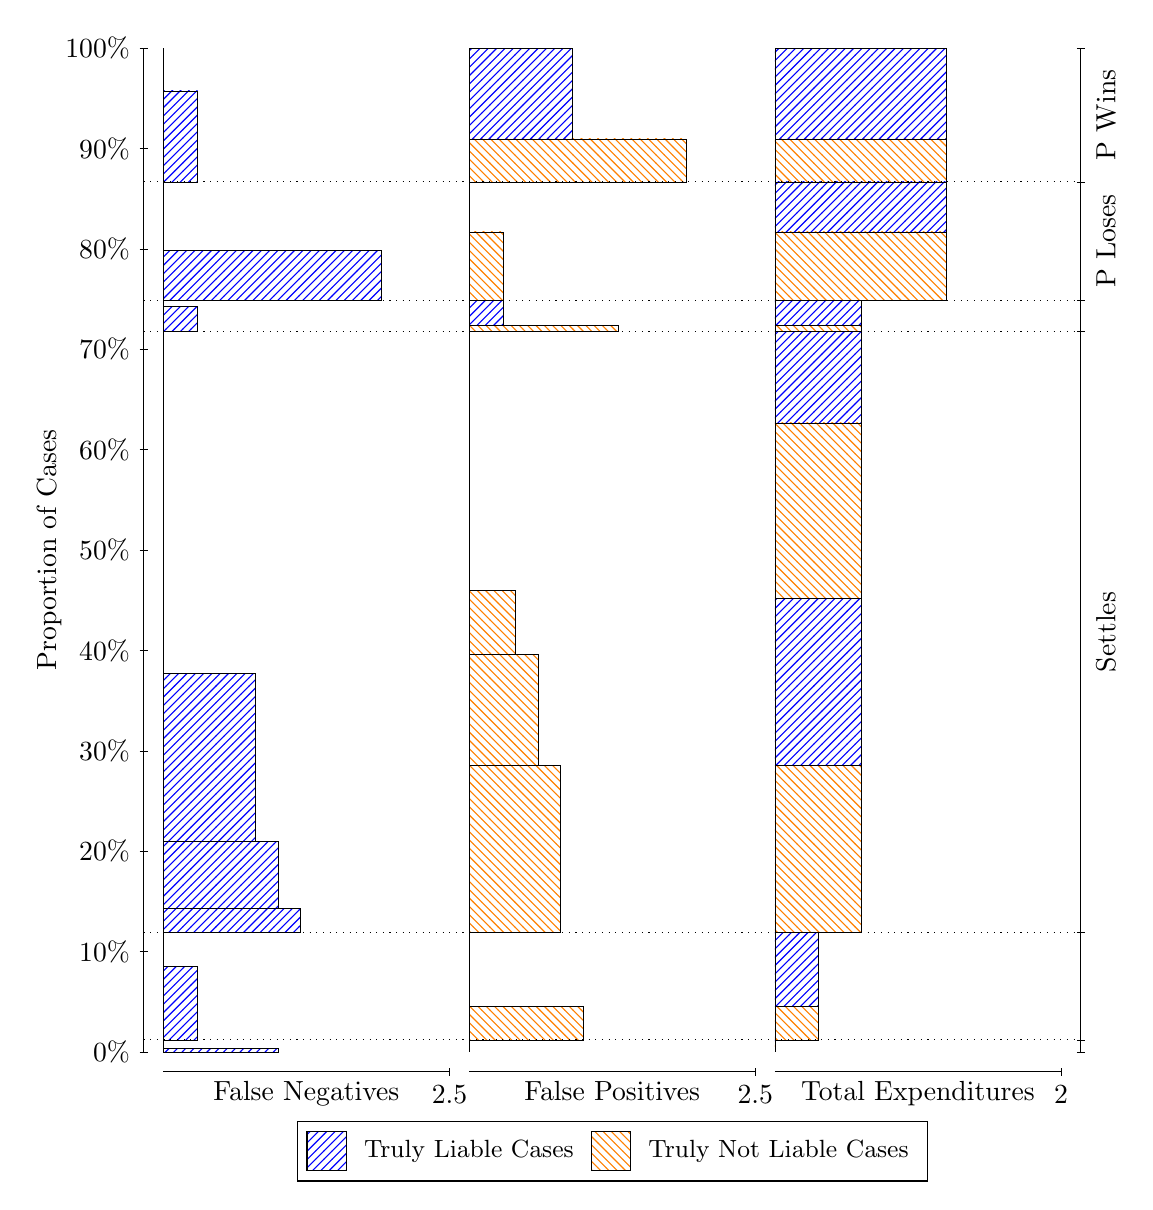
\begin{tikzpicture}
\draw[black, very thin] (1.5,1.75) -- (1.5,14.5);
\node[rotate=90, text=black, anchor=center] at (0.3, 8.125) {Proportion of Cases};
\draw[black, very thin] (1.45,1.75) -- (1.55,1.75);
\node[text=black, anchor=east] at (1.45, 1.75) {0\%};
\draw[black, very thin] (1.45,3.025) -- (1.55,3.025);
\node[text=black, anchor=east] at (1.45, 3.025) {10\%};
\draw[black, very thin] (1.45,4.3) -- (1.55,4.3);
\node[text=black, anchor=east] at (1.45, 4.3) {20\%};
\draw[black, very thin] (1.45,5.575) -- (1.55,5.575);
\node[text=black, anchor=east] at (1.45, 5.575) {30\%};
\draw[black, very thin] (1.45,6.85) -- (1.55,6.85);
\node[text=black, anchor=east] at (1.45, 6.85) {40\%};
\draw[black, very thin] (1.45,8.125) -- (1.55,8.125);
\node[text=black, anchor=east] at (1.45, 8.125) {50\%};
\draw[black, very thin] (1.45,9.4) -- (1.55,9.4);
\node[text=black, anchor=east] at (1.45, 9.4) {60\%};
\draw[black, very thin] (1.45,10.675) -- (1.55,10.675);
\node[text=black, anchor=east] at (1.45, 10.675) {70\%};
\draw[black, very thin] (1.45,11.95) -- (1.55,11.95);
\node[text=black, anchor=east] at (1.45, 11.95) {80\%};
\draw[black, very thin] (1.45,13.225) -- (1.55,13.225);
\node[text=black, anchor=east] at (1.45, 13.225) {90\%};
\draw[black, very thin] (1.45,14.5) -- (1.55,14.5);
\node[text=black, anchor=east] at (1.45, 14.5) {100\%};

\draw[black, very thin] (13.4,1.75) -- (13.4,14.5);
\draw[black, very thin] (13.35,1.75) -- (13.45,1.75);
\node[anchor=west] at (13.35, 1.75) {};
\draw[black, very thin] (13.35,1.904) -- (13.45,1.904);
\node[anchor=west] at (13.35, 1.904) {};
\draw[black, very thin] (13.35,3.2649) -- (13.45,3.2649);
\node[anchor=west] at (13.35, 3.2649) {};
\draw[black, very thin] (13.35,10.901) -- (13.45,10.901);
\node[anchor=west] at (13.35, 10.901) {};
\draw[black, very thin] (13.35,11.296) -- (13.45,11.296);
\node[anchor=west] at (13.35, 11.296) {};
\draw[black, very thin] (13.35,12.801) -- (13.45,12.801);
\node[anchor=west] at (13.35, 12.801) {};
\draw[black, very thin] (13.35,14.5) -- (13.45,14.5);
\node[anchor=west] at (13.35, 14.5) {};

\draw[black, very thin, pattern color=blue, pattern=north east lines] (1.75,1.75) rectangle (3.2033,1.7923);
\draw[black, very thin, pattern color=orange, pattern=north west lines] (1.75,1.7923) rectangle (1.75,1.904);
\draw[black, very thin, pattern color=blue, pattern=north east lines] (1.75,1.904) rectangle (2.186,2.839);
\draw[black, very thin, pattern color=orange, pattern=north west lines] (1.75,2.839) rectangle (1.75,3.2649);
\draw[black, very thin, pattern color=blue, pattern=north east lines] (1.75,3.2649) rectangle (3.494,3.576);
\draw[black, very thin, pattern color=blue, pattern=north east lines] (1.75,3.576) rectangle (3.2033,4.4281);
\draw[black, very thin, pattern color=blue, pattern=north east lines] (1.75,4.4281) rectangle (2.9127,6.5531);
\draw[black, very thin, pattern color=orange, pattern=north west lines] (1.75,6.5531) rectangle (1.75,10.901);
\draw[black, very thin, pattern color=blue, pattern=north east lines] (1.75,10.901) rectangle (2.186,11.219);
\draw[black, very thin, pattern color=orange, pattern=north west lines] (1.75,11.219) rectangle (1.75,11.296);
\draw[black, very thin, pattern color=blue, pattern=north east lines] (1.75,11.296) rectangle (4.5113,11.933);
\draw[black, very thin, pattern color=orange, pattern=north west lines] (1.75,11.933) rectangle (1.75,12.801);
\draw[black, very thin, pattern color=blue, pattern=north east lines] (1.75,12.801) rectangle (2.186,13.957);
\draw[black, very thin, pattern color=orange, pattern=north west lines] (1.75,13.957) rectangle (1.75,14.5);
\draw[black, very thin, pattern color=orange, pattern=north west lines] (5.6333,1.75) rectangle (5.6333,1.8617);
\draw[black, very thin, pattern color=blue, pattern=north east lines] (5.6333,1.8617) rectangle (5.6333,1.904);
\draw[black, very thin, pattern color=orange, pattern=north west lines] (5.6333,1.904) rectangle (7.0867,2.33);
\draw[black, very thin, pattern color=blue, pattern=north east lines] (5.6333,2.33) rectangle (5.6333,3.2649);
\draw[black, very thin, pattern color=orange, pattern=north west lines] (5.6333,3.2649) rectangle (6.796,5.3899);
\draw[black, very thin, pattern color=orange, pattern=north west lines] (5.6333,5.3899) rectangle (6.5053,6.8027);
\draw[black, very thin, pattern color=orange, pattern=north west lines] (5.6333,6.8027) rectangle (6.2147,7.6132);
\draw[black, very thin, pattern color=blue, pattern=north east lines] (5.6333,7.6132) rectangle (5.6333,10.901);
\draw[black, very thin, pattern color=orange, pattern=north west lines] (5.6333,10.901) rectangle (7.5227,10.979);
\draw[black, very thin, pattern color=blue, pattern=north east lines] (5.6333,10.979) rectangle (6.0693,11.296);
\draw[black, very thin, pattern color=orange, pattern=north west lines] (5.6333,11.296) rectangle (6.0693,12.165);
\draw[black, very thin, pattern color=blue, pattern=north east lines] (5.6333,12.165) rectangle (5.6333,12.801);
\draw[black, very thin, pattern color=orange, pattern=north west lines] (5.6333,12.801) rectangle (8.3947,13.345);
\draw[black, very thin, pattern color=blue, pattern=north east lines] (5.6333,13.345) rectangle (6.9413,14.5);
\draw[black, very thin, pattern color=orange, pattern=north west lines] (9.5167,1.75) rectangle (9.5167,1.8617);
\draw[black, very thin, pattern color=blue, pattern=north east lines] (9.5167,1.8617) rectangle (9.5167,1.904);
\draw[black, very thin, pattern color=orange, pattern=north west lines] (9.5167,1.904) rectangle (10.062,2.33);
\draw[black, very thin, pattern color=blue, pattern=north east lines] (9.5167,2.33) rectangle (10.062,3.2649);
\draw[black, very thin, pattern color=orange, pattern=north west lines] (9.5167,3.2649) rectangle (10.607,5.3899);
\draw[black, very thin, pattern color=blue, pattern=north east lines] (9.5167,5.3899) rectangle (10.607,7.5149);
\draw[black, very thin, pattern color=orange, pattern=north west lines] (9.5167,7.5149) rectangle (10.607,9.7382);
\draw[black, very thin, pattern color=blue, pattern=north east lines] (9.5167,9.7382) rectangle (10.607,10.901);
\draw[black, very thin, pattern color=orange, pattern=north west lines] (9.5167,10.901) rectangle (10.607,10.979);
\draw[black, very thin, pattern color=blue, pattern=north east lines] (9.5167,10.979) rectangle (10.607,11.296);
\draw[black, very thin, pattern color=orange, pattern=north west lines] (9.5167,11.296) rectangle (11.697,12.165);
\draw[black, very thin, pattern color=blue, pattern=north east lines] (9.5167,12.165) rectangle (11.697,12.801);
\draw[black, very thin, pattern color=orange, pattern=north west lines] (9.5167,12.801) rectangle (11.697,13.345);
\draw[black, very thin, pattern color=blue, pattern=north east lines] (9.5167,13.345) rectangle (11.697,14.5);
\draw[black, dotted] (1.5,1.904) -- (13.4,1.904);
\draw[black, dotted] (1.5,3.2649) -- (13.4,3.2649);
\draw[black, dotted] (1.5,10.901) -- (13.4,10.901);
\draw[black, dotted] (1.5,11.296) -- (13.4,11.296);
\draw[black, dotted] (1.5,12.801) -- (13.4,12.801);
\draw[black, very thin] (1.75,1.5) -- (5.3833,1.5);
\node[text=black, anchor=north] at (3.5667, 1.5) {False Negatives};
\draw[black, very thin] (5.3833,1.45) -- (5.3833,1.55);
\node[text=black, anchor=north] at (5.3833, 1.45) {2.5};

\draw[black, very thin] (5.6333,1.5) -- (9.2667,1.5);
\node[text=black, anchor=north] at (7.45, 1.5) {False Positives};
\draw[black, very thin] (9.2667,1.45) -- (9.2667,1.55);
\node[text=black, anchor=north] at (9.2667, 1.45) {2.5};

\draw[black, very thin] (9.5167,1.5) -- (13.15,1.5);
\node[text=black, anchor=north] at (11.333, 1.5) {Total Expenditures};
\draw[black, very thin] (13.15,1.45) -- (13.15,1.55);
\node[text=black, anchor=north] at (13.15, 1.45) {2};



\node[text=black, centered, rotate=90] at (13.72, 7.0831) {Settles};

\node[text=black, centered, rotate=90] at (13.72, 12.049) {P Loses};
\node[text=black, centered, rotate=90] at (13.72, 13.651) {P Wins};

\draw (7.449999999999999,1.5) node[draw=none] (baseCoordinate) {};
\begin{scope}[align=center]
        \matrix[scale=0.5, draw=black, below=0.5cm of baseCoordinate, nodes={draw}, column sep=0.1cm]{
            \node[rectangle, draw, minimum width=0.5cm, minimum height=0.5cm, pattern color=blue, pattern=north east lines] {}; &
            \node[draw=none, font=\small, text=black] (B) {Truly Liable Cases}; &
            \node[rectangle, draw, minimum width=0.5cm, minimum height=0.5cm, pattern color=orange, pattern=north west lines] {}; &
            \node[draw=none, font=\small, text=black] (B) {Truly Not Liable Cases}; \\
            };
\end{scope}

\end{tikzpicture}
\end{document}